\documentclass[a4paper,11pt,fleqn,twoside,openright]{memoir} % Brug openright hvis chapters skal starte p� h�jresider; openany, oneside
%\usepackage{fancyhdr}%mega nemt sidehoved/fod%virker ikke med memoir �benbart
%%%% PACKAGES %%%%

%\usepackage[T1]{fontenc}
%\usepackage{pgfplots}%Ting til grafer (sat ind december 2012)
%\pgfplotsset{
%  compat=newest,
%  xlabel near ticks,
%  ylabel near ticks
%} Ting til grafer (sat ind december 2012)

\usepackage[english]{babel}							% Dansk sporg, f.eks. tabel, figur og kapitel
%\usepackage{pst-plot,pst-node}
%\usepackage[pdf]{pstricks} % G�r det muligt at tegne vektor grafik.
\usepackage{auto-pst-pdf,pstricks-add}
% �� Overs�ttelse og tegns�tning �� %
%\usepackage[ansinew]{inputenc}					% G�r det muligt at bruge �, � og � i sine .tex-filer

%\usepackage[T1]{fontenc}								% Hj�lper med orddeling ved �, � og �. S�tter fontene til at v�re ps-fonte, i stedet for bmp					

% �� FONTS �� % LaTeX er fanme ringe til skrifttyper!
%\usepackage{txfonts}									% konflikter med et eller andet.. giver i hvert fald fejl
\usepackage{mathptmx}								% times (den vi normalt bruger - bare ingen fed mat skrift)
%\usepackage{fourier}									% s�dan lidt middle ground mellem times og pazo (har heller ikke mathbf)
%\usepackage{mathpazo}								% Har fed tekst i matematik (minus mathbf), grim almindelig skrift
%\usepackage{mtpro2}									% f�lger ikke med som standard, men hvis nogen kan installere det skal de da v�re velkomne

\usepackage{latexsym}										% LaTeX symboler
\usepackage{xcolor,ragged2e,fix-cm}			% Justering af elementer
\usepackage{pdfpages}										% G�r det muligt at inkludere pdf-dokumenter med kommandoen \includepdf[pages={x-y}]{fil.pdf}	
\pretolerance=2500 											% G�r det muligt at justre afstanden med ord (h�jt tal, mindre orddeling og mere space mellem ord)
\usepackage{ulem}                       % Gennemstregning af ord med koden \sout{}
\usepackage{fixltx2e}										% Retter forskellige bugs i LaTeX-kernen
\usepackage[shortlabels]{enumitem}			% Muligg�r enkelt konfiguration af lister
\usepackage{alltt}											% Bruges af highlighting (matlab kode)
%\usepackage{Lastpage}

%Matlab kode hightlighting
 \definecolor{string}{rgb}{0.7,0.0,0.0}
    \definecolor{comment}{rgb}{0.13,0.54,0.13}
    \definecolor{keyword}{rgb}{0.0,0.0,1.0}
											
%Include cpp coding in text
\usepackage{listings}
\usepackage{color}

\definecolor{dkgreen}{rgb}{0,0.6,0}
\definecolor{gray}{rgb}{0.5,0.5,0.5}
\definecolor{mauve}{rgb}{0.58,0,0.82}

\lstset{frame=tb,
  language=C++,  
  aboveskip=3mm,
  belowskip=3mm,
  showstringspaces=false,
  columns=flexible,
  basicstyle={\small\ttfamily},
  numbers=none,
  numberstyle=\tiny\color{gray},
  keywordstyle=\color{blue},
  commentstyle=\color{dkgreen},
  stringstyle=\color{mauve},
  breaklines=true,
  breakatwhitespace=true,
  tabsize=3
}											
																			
% �� Figurer og tabeller � floats  �� %
\usepackage{flafter}										% S�rger for at dine floats ikke optr�der i teksten f�r de er sat ind.
\usepackage{multirow}                		% Fletning af r�kker
\usepackage{hhline}                   	% Dobbelte horisontale linier
\usepackage{multicol}         	        % Fletning af kolonner
\usepackage{colortbl} 									% Mulig�re farver i tabeller
\usepackage{rotating}										% Muligg�r rotation af tekst i tabeller med \begin{sideways}...\end{sideways}
\usepackage{wrapfig}										% Inds�ttelse af figurer omsv�bt af tekst. \begin{wrapfigure}{Placering}{St�rrelse}
\usepackage{graphicx} 									% Pakke til jpeg/png billeder
%\pdfoptionpdfminorversion=6%							% Muligg�r inkludering af pdf dokumenter, af version 1.6 og h�jere
\usepackage{tabularx} %Muligg�r at man kan str�kke en tabel-kolonne til �nsket l�ngde
\newsubfloat{figure}
\usepackage{epstopdf}

% �� Matematiske formler og maskinkode ��
\usepackage{amsmath, amssymb} 	% Bedre matematik og ekstra fonte 
\usepackage{textcomp}                 	% Adgang til tekstsymboler
\usepackage{mathtools}									% Udvidelse af amsmath-pakken. 
\usepackage{eso-pic}										% Tilf�j billedekommandoer p� hver side
\usepackage{lipsum}											% Dummy text \lipsum[..]



% �� Referencer, bibtex og url'er �� %
\usepackage{url}												% Til at s�tte urler op med. Virker sammen med hyperref
\usepackage[english]{varioref}						% Giver flere bedre mulighed for at lave krydshenvisninger
%\usepackage{natbib}											% Litteraturliste med forfatter-�r og nummerede referencer
%\usepackage{cite} 												% G�r det muligt at nummere kilder
\usepackage{xr}													% Referencer til eksternt dokument med \externaldocument{<NAVN>}
\usepackage{nomencl}										% Pakke til at danne nomenklaturliste
\makenomenclature												% Nomenklaturliste


% �� Floats �� %
\let\newfloat\relax 										% Memoir har allerede defineret denne, men det g�r float pakken ogs�
\usepackage{float}

\usepackage[footnote,draft,english,silent,nomargin]{fixme}		% Inds�t rettelser og lignende med \fixme{...} Med final i stedet for draft, udl�ses en error 																															for hver fixme, der ikke er slettet, n�r rapporten bygges.

%%%% CUSTOM SETTINGS %%%%

% �� Marginer �� %
\setlrmarginsandblock{3.5cm}{2.5cm}{*}	% \setlrmarginsandblock{Indbinding}{Kant}{Ratio}
\setulmarginsandblock{2.5cm}{3.0cm}{*}	% \setulmarginsandblock{Top}{Bund}{Ratio}
\checkandfixthelayout 									% Laver forskellige beregninger og s�tter de almindelige l�ngder op til brug ikke memoir pakker

%	�� Afsnitsformatering �� %
\setlength{\parindent}{0mm}           	% St�rrelse af indryk
\setlength{\parskip}{4mm}          			% Afstand mellem afsnit ved brug af double Enter
\linespread{1,1}												% Linie afstand

% �� Litteraturlisten �� %
%\bibpunct[,]{[}{]}{;}{a}{,}{,} 					% Definerer de 6 parametre ved Harvard henvisning (bl.a. parantestype og seperatortegn)
%\bibliographystyle{bibtex/harvard}			% Udseende af litteraturlisten. Ligner dk-apali - mvh Klein

% �� Indholdsfortegnelse �� %
\setsecnumdepth{subsection}		 					% Dybden af nummerede overkrifter (part/chapter/section/subsection)
\maxsecnumdepth{subsection}							% �ndring af dokumentklassens gr�nse for nummereringsdybde
\settocdepth{subsection} 								% Dybden af indholdsfortegnelsen

% �� Lister �� %
\setlist{
  topsep=-1ex,														% Vertikal afstand mellem tekst og listen
  itemsep=-1ex,													% Vertikal afstand mellem items
  partopsep=-0ex,
  parsep=1ex
} 

% �� Visuelle referencer �� %
\usepackage[colorlinks]{hyperref}			 	% Giver mulighed for at ens referencer bliver til klikbare hyperlinks. .. [colorlinks]{..}
\hypersetup{pdfborder = 0}							% Fjerner ramme omkring links i fx indholsfotegnelsen og ved kildehenvisninger ��
\hypersetup{														%	Ops�tning af farvede hyperlinks
    colorlinks = false,
    linkcolor = black,
    anchorcolor = black,
    citecolor = black
}

\definecolor{gray}{gray}{0.80}					% Definerer farven gr�

% �� Ops�tning af figur- og tabeltekst �� %
 	\captionnamefont{
 		\small\bfseries\itshape}						% Ops�tning af tekstdelen ("Figur" eller "Tabel")
  \captiontitlefont{\small}							% Ops�tning af nummerering
  \captiondelim{. }											% Seperator mellem nummerering og figurtekst
  \hangcaption													%	Venstrejusterer flere-liniers figurtekst under hinanden
  \captionwidth{\linewidth}							% Bredden af figurteksten
	\setlength{\belowcaptionskip}{-15pt}		% Afstand under figurteksten
		
% �� Navngivning �� %
\addto\captionsenglish{
	\renewcommand\appendixname{Appendix}
	\renewcommand\contentsname{Table of Contents}	
	\renewcommand\appendixpagename{Appendix}
	\renewcommand\cftchaptername{\chaptername~}				% Skriver "Kapitel" foran kapitlerne i indholdsfortegnelsen
	\renewcommand\cftappendixname{\appendixname~}			% Skriver "Bilag" foran bilagene i indholdsfortegnelsen
	\renewcommand\appendixtocname{Appendix}
}

% �� Kapiteludssende �� %


\definecolor{numbercolor}{gray}{0.7}			% Definerer en farve til brug til kapiteludseende
\newif\ifchapternonum

\makechapterstyle{jenor}{									% Definerer kapiteludseende -->
  \renewcommand\printchaptername{}
  \renewcommand\printchapternum{}
  \renewcommand\printchapternonum{\chapternonumtrue}
  \renewcommand\chaptitlefont{\fontfamily{pbk}\fontseries{db}\fontshape{n}\fontsize{25}{35}\selectfont\raggedleft}
  \renewcommand\chapnumfont{\fontfamily{pbk}\fontseries{m}\fontshape{n}\fontsize{1in}{0in}\selectfont\color{numbercolor}}
  \renewcommand\printchaptertitle[1]{%
    \noindent
    \ifchapternonum
    \begin{tabularx}{\textwidth}{X}
    {\let\\\newline\chaptitlefont ##1\par} 
    \end{tabularx}
    \par\vskip-2.5mm\hrule
    \else
    \begin{tabularx}{\textwidth}{Xl}
    {\parbox[b]{\linewidth}{\chaptitlefont ##1}} & \raisebox{-15pt}{\chapnumfont \thechapter}
    \end{tabularx}
    \par\vskip2mm\hrule
    \fi
  }
}																						% <--

%BLUEBOX KAPITEL
\newsavebox{\ChpNumBox}
\definecolor{ChapBlue}{rgb}{1,0,0} % !!
\makeatletter
\newcommand*{\thickhrulefill}{%
\leavevmode\leaders\hrule height 1\p@ \hfill \kern \z@}
\newcommand*\BuildChpNum[2]{%
\begin{tabular}[t]{@{}c@{}}
\makebox[0pt][c]{#1\strut} \\[.5ex]
\colorbox{ChapBlue}{%
\rule[-10em]{0pt}{0pt}%
\rule{1ex}{0pt}\color{black}#2\strut
\rule{1ex}{0pt}}%
\end{tabular}}
\makechapterstyle{BlueBox}{%
\renewcommand{\chapnamefont}{\large\scshape}
\renewcommand{\chapnumfont}{\Huge\bfseries} 		
\renewcommand{\chaptitlefont}{\raggedright\Huge\scshape} % \bfseries
\setlength{\beforechapskip}{10pt}	%DEFAULT:20pt
\setlength{\midchapskip}{20pt}	%DEFAULT:26pt
\setlength{\afterchapskip}{15pt}	%DEFAULT:40pt !!
\renewcommand{\printchaptername}{}
\renewcommand{\chapternamenum}{}
\renewcommand{\printchapternum}{%
\sbox{\ChpNumBox}{%
\BuildChpNum{\chapnamefont\@chapapp}%
{\chapnumfont\thechapter}}}
\renewcommand{\printchapternonum}{%
\sbox{\ChpNumBox}{%
\BuildChpNum{\chapnamefont\vphantom{\@chapapp}}%
{\chapnumfont\hphantom{\thechapter}}}}
\renewcommand{\afterchapternum}{}
\renewcommand{\printchaptertitle}[1]{%
\usebox{\ChpNumBox}\hfill
\parbox[t]{\hsize-\wd\ChpNumBox-1em}{%
\vspace{\midchapskip}%
\thickhrulefill\par
\chaptitlefont ##1\par}}%
}


% Valg af kapiteludseende - dette kan udskiftes efter �nske
%\chapterstyle{madsen}	%P1-style		
\chapterstyle{BlueBox}									

% �� Sidehoved �� %

\makepagestyle{custom}		% Definerer sidehoved og sidefod - kan modificeres efter �nske -->
\makepsmarks{custom}{																						
\def\chaptermark##1{\markboth{\itshape\thechapter. ##1}{}}		% Henter kapitlet den p�g�ldende side h�rer under med kommandoen \leftmark. \itshape g�r teksten kursiv
\def\sectionmark##1{\markright{\thesection. ##1}{}}					% Henter afsnittet den p�g�ldende side h�rer under med kommandoen \rightmark
}																														% Sidetallet skrives med kommandoen \thepage	
\makeevenhead{custom}{Computational Physics}{}{\leftmark}							% Definerer lige siders sidehoved efter modellen \makeevenhead{Navn}{Venstre}{Center}{H�jre}
\makeoddhead{custom}{\rightmark}{}{University of Oslo}			% Definerer ulige siders sidehoved efter modellen \makeoddhead{Navn}{Venstre}{Center}{H�jre}
\makeevenfoot{custom}{\thepage}{}{}													% Definerer lige siders sidefod efter modellen \makeevenfoot{Navn}{Venstre}{Center}{H�jre}
\makeoddfoot{custom}{}{}{\thepage}														% Definerer ulige siders sidefod efter modellen \makeoddfoot{Navn}{Venstre}{Center}{H�jre}		
\makeheadrule{custom}{\textwidth}{0.5pt}											% Tilf�jer en streg under sidehovedets indhold
\makefootrule{custom}{\textwidth}{0.5pt}{1mm}								% Tilf�jer en streg under sidefodens indhold

\copypagestyle{nychapter}{custom}														% F�lgende linier s�rger for, at sidefoden bibeholdes p� kapitlets f�rste side
\makeoddhead{nychapter}{}{}{}
\makeevenhead{nychapter}{}{}{}
\makeheadrule{nychapter}{\textwidth}{0pt}
\aliaspagestyle{chapter}{nychapter}													% <--

\pagestyle{custom} %normalt plain% Valg af sidehoved og sidefod
\usepackage[left=2.4cm, right=2.4cm, top=3cm, bottom=3cm]{geometry}	%Overrider tidliger marginer - men det er lidt mere simpelt.

%%%% CUSTOM COMMANDS %%%%
%referencer
\newcommand{\figref}[1]{Fig.~\ref{#1}}
\newcommand{\tabref}[1]{Tab.~\ref{#1}}	
\newcommand{\matref}[1]{Eq.~\eqref{#1}}
\newcommand{\chapref}[1]{Chap.~\ref{#1}}
\newcommand{\secref}[1]{Sec.~\ref{#1}}
\newcommand{\subsecref}[1]{Subsec.~\ref{#1}}
\newcommand{\appref}[1]{App.~\ref{#1}}
\newcommand{\citer}[1]{\citep[Se][]{#1}}
\newcommand{\citerk}[2][]{\citep[Se][kap.~#1]{#2}}
\newcommand{\citers}[2][]{\citep[Se][s.~#1]{#2}}


% �� Billede hack �� %
\newcommand{\figur}[4]{
		\begin{figure}[H] \centering
			\includegraphics[width=#1\textwidth]{billeder/#2}
			\caption{#3}\label{#4}
		\end{figure} 
		}
		
% �� Specielle tegn �� %
\newcommand{\grader}{\ensuremath{^{\circ}\text{C}}}
\newcommand{\gr}{\ensuremath{^{\circ}}}
\newcommand{\g}{\cdot}


% �� Promille-hack (\promille) �� %
\newcommand{\promille}{%
  \relax\ifmmode\promillezeichen
        \else\leavevmode\(\mathsurround=0pt\promillezeichen\)\fi}
\newcommand{\promillezeichen}{%
  \kern-.05em%
  \raise.5ex\hbox{\the\scriptfont0 0}%
  \kern-.15em/\kern-.15em%
  \lower.25ex\hbox{\the\scriptfont0 00}}

\newcommand{\HRule}{\rule{\linewidth}{0.5mm}}

% �� CUSTOM MATEMATIK/FYSIK-TING ��
\renewcommand{\v}[1]{\ensuremath{\mbox{\textbf{#1}}}} % for vectors
\newcommand{\gv}[1]{\ensuremath{\mbox{\boldmath$ \vec{#1}  $}}} 
% for vectors of Greek letters
\newcommand{\uv}[1]{\ensuremath{\mbox{\boldmath$ \hat{#1}  $}}}  % for unit vector
\newcommand{\abs}[1]{\left| #1 \right|} % for absolute value
\newcommand{\avg}[1]{\left< #1 \right>} % for average
\let\underdot=\d % rename builtin command \d{} to \underdot{}
\renewcommand{\d}[2]{\frac{d #1}{d #2}} % for derivatives
\newcommand{\dd}[2]{\frac{d^2 #1}{d #2^2}} % for double derivatives
\newcommand{\pd}[2]{\frac{\partial #1}{\partial #2}} 
% for partial derivatives
\newcommand{\pdd}[2]{\frac{\partial^2 #1}{\partial #2^2}} 
% for double partial derivatives
\newcommand{\pdc}[3]{\left( \frac{\partial #1}{\partial #2}
 \right)_{#3}} % for thermodynamic partial derivatives
\newcommand{\ket}[1]{\left| #1 \right>} % for Dirac bras
\newcommand{\bra}[1]{\left< #1 \right|} % for Dirac kets
\newcommand{\braket}[2]{\left< #1 \vphantom{#2} \right|
 \left. #2 \vphantom{#1} \right>} % for Dirac brackets
\newcommand{\matrixel}[3]{\left< #1 \vphantom{#2#3} \right|
 #2 \left| #3 \vphantom{#1#2} \right>} % for Dirac matrix elements
\newcommand{\grad}[1]{\gv{\nabla} #1} % for gradient
\let\divsymb=\div % rename builtin command \div to \divsymb
\renewcommand{\div}[1]{\gv{\nabla} \cdot #1} % for divergence
\newcommand{\curl}[1]{\gv{\nabla} \times #1} % for curl
\let\baraccent=\= % rename builtin command \= to \baraccent
\renewcommand{\=}[1]{\stackrel{#1}{=}} % for putting numbers above =
\renewcommand\Re{\operatorname{Re}}
\renewcommand\Im{\operatorname{Im}}
\newcommand{\comp}[1]{\widetilde{#1}}
\newcommand{\unit}[1]{\ensuremath{\, \mathrm{#1}}}

\newcommand{\eqvref}[1]{(\ref{#1}) p� side \pageref{#1}}

\newcommand{\forsog}[1]{\underline{#1}}

\newcommand{\superscript}[1]{\ensuremath{^{\textrm{#1}}}}
\newcommand{\subscript}[1]{\ensuremath{_{\textrm{#1}}}}


%%%% ORDDELING %%%%

\hyphenation{egen-skab-er egen-skab hvad hvem hvor Halv-le-der-ud-snit-tet}

% Makro til fxnotes
\newcommand{\AVP}[1]{\fxnote{\textbf{AVP}: #1}}
\newcommand{\BM}[1]{\fxnote{\textbf{BM}: #1}}
\newcommand{\flops}[1]{flops}
\raggedbottom
\begin{document}

\frontmatter	% Romertal på de første sider
\thispagestyle{empty}

\begin{center}


% Upper part of the page

\textsc{\LARGE University of Oslo}\\[0.5cm]

\textsc{\Large Computational Physics}\\[2cm]
 

% Title
\HRule \\[0.4cm]
 \LARGE \textbf{Project 4}  \\[0.2cm]
\HRule \\[2.5cm]

\vspace{2cm}

\includegraphics[width=0.8\textwidth]{Figures/UiO_Seal_A_ENG.png}\\  %Forsidebillede

\vfill 
 
% Forfattere og vejleder
\begin{tabularx}{\textwidth}{l X r}
\hline
& & \large \emph{Authors:}\\
& & \large Birgitte Madsen\\
& & \large Magnus Isaksen \\
& & \large Soumya Chalakkal \\
\hline

\end{tabularx}




\vfill

% Bottom of the page
{\large Autumn 2015}

\end{center}
\cleardoublepage


\cleardoublepage		
% Dette er LaTeX-versionen af titelbladet for tek-nat-basis-rapporter 2004 efterår
% Filen kræver:
% Universitetets logo:  aau-logo.png (for LaTeX) eller aau-logo.ps (for LaTeX)
% Synopsis: En fil ved navn synopsis.tex

% Udarbejdet af: Hans HŸttel (hans@cs.auc.dk) 21. maj 2003
% Rettet af Morten Christophersen (mortench@tnb.aau.dk) 30. nov 2004(ændret til nyt design 2004 efterår)

%\documentclass[11pt]{article}
%\ifx\pdfoutput\undefined 
%\usepackage[dvips]{graphicx}
%\else
%\usepackage[pdftex]{graphicx} 
%\usepackage{type1cm} \fi
%    \usepackage[ansinew]{inputenc}
%    \usepackage{a4}

%\begin{document} 
\phantomsection
\pdfbookmark[0]{Titelblad}{titelblad}
\thispagestyle{empty}
%\begin{titlepage}
\begin{nopagebreak}
{\samepage 
\begin{tabular}{r}
\parbox{\textwidth}{  \raisebox{1mm}{
\includegraphics[height=1.5cm]{Figures/UiO_Seal_A_ENG.png}}
\hfill \parbox{5.5cm}{\begin{tabular}{r} %4.90
{\small \textbf{Department of Physics}}\\
{\small  \textbf{University of Oslo}} \\
{\small  Sem S\ae lands vei 24} \\
{\small  0371 Oslo, Norway} \\
{\small +47 22 85 64 28} \\
%{\small Fax 99 40 92 35} \\
{\small http://www.mn.uio.no/fysikk/english/}
\end{tabular}}}

\end{tabular}

\vspace{2.5cm}
\begin{tabular}{cc}
\parbox{20cm}{
\begin{description}
\item { \textbf{Course:}}

	Computational Physics\\
	\hspace{4cm}
	\vspace{0.7cm}
\item { \textbf{Project number:}}

	4 \\
	\hspace{4cm}
	\vspace{0.7cm}

\item {\textbf{Link to GitHub folder:} }

	\url{https://} ???????????? \\ 
	\hspace{4cm}
	\vspace{0.7cm}

\item { \textbf{Hand-in deadline:}}

   Friday, November 13, 2015\\
  \hspace{4cm}
  \vspace{0.7cm}
  
\item { \textbf{Project Members:}}

Birgitte Madsen \\
Magnus Isaksen \\
Soumya Chalakkal \\
  \hspace{2cm}
  \vspace{0.7cm}

\end{description}

\vspace{0.25cm}
\begin{description}
\item { \textbf{Copies:} 1}
\item { \textbf{Page count:} ????????  } 
\item { \textbf{Appendices:} 0} 
\item { \textbf{Completed:} ????????? } 
\end{description}
\vfill } &
%\parbox{7cm}{
%  \vspace{.15cm}
%  \hfill 
%  \begin{tabular}{l}
%  {\textbf{Synopsis:}}\bigskip \\
%  \fbox{
%    \parbox{6.5cm}{\bigskip
%     {\vfill{\small \input{Chapters/Formalia/synopsis.tex}
%     \bigskip}}
%     }}
%   \end{tabular}}
\end{tabular}}
\\ \\ \\ 

\noindent{\footnotesize{\textit{The content of the report is freely available, but publication (with source) may only be made with the agreement of the authors.}}}
\end{nopagebreak}
%\end{titlepage}
%\end{document}

\cleardoublepage
\chapter*{Abstract}
\fxnote{write abstract}
\cleardoublepage	
%\chapter*{Preface}
This project is written by 6th semester physics group 4.207a at the Department of Physics and
Nanotechnology at Aalborg University, Denmark, in the Spring semester, 2014, as a 10 ECTS-point bachelor project.

\subsection*{Reading Guide}
Succeeding chapters support each other, and it is therefore recommended to read the report chronologically.
When referring to equations or the like in the text, \textit{equation} will be shortened Eq., \textit{table} will be shortened Tab., and so forth.
In \appref{app:ListOfSymbols} a list of frequently used symbols and constants are given.
The external references used in this work appear in numbered order in brackets in the text and are listed in the bibliography at the end of the report in order of succession.

\subsection*{Signatures}
The group member's signatures below express that the entire group is accountable for all aspects of the project and all chapters of the report. 

\vspace{4cm}

\begin{table}[H]
	\centering
		\begin{tabular}{c c}
			\underline{\phantom{JAERJAERJAERJAERJAERJAERJAER}}	 	&	\underline{\phantom{JAERJAERJAERJAERJAERJAERJAER}} 
			\\
			Andreas V. Pedersen								& 	Birgitte Madsen	
			\\									
		\end{tabular}
\end{table}
%\cleardoublepage			
\tableofcontents*

\mainmatter % Side nummereringen starter ved 1 herfra

	\chapter{Introduction}
%An introduction where you explain the aims and rationale for the physics case and what you have done. At the end of the introduction you should give a brief summary of the structure of the report

Awesome introduction!!!!!
	\chapter{Method}
\label{chap:method} 
Write awesome introduction

The source codes for the algorithms described in this chapter can be found in the Github folder \url{https://}.  
\fxnote{fix lines!}

	\section{Nature of the problem}
\label{sec:NatureOfTheProblem}
%Give a short description of the nature of the problem and the eventual numerical methods, you have used.
%"Non-computational" algebra
%Show that you can rewrite this equation as a linear set of equations of the form
This problem also have a nature!!





	\subsection{Determining Quantities}
\label{sec:DeterminingQuantities}
For the canonical ensemble with probability distribution given by the Boltzmann distribution
\begin{align}
	P_i (\beta ) = \frac{e^{-\beta E_i}}{Z}
	\label{eq:BoltzmannDistribution}
\end{align}  
with $\beta = 1/k_B T$, in which $k_B$ is Boltzmann's constant and $T$ is the temperature of the system, $E_i$ being the energy of the $i$'th microstate, and $Z$ being the partition function given by
\begin{align}
	Z = \sum _{i=1} ^M e^{-\beta E_i}
	\label{eq:PartitionFunction}
\end{align}  
for a system with $M$ microstates. 
For each microstate $i$ in a spin system with $N$ spins $s_i = \pm 1$, the energy $E_i$ and magnetization $\mathcal{M}_i$ are given as
\fxnote{what is J ?!}
\begin{align}
	E_i = -J \sum_{<kl>} ^N s_k s_l 
	\qquad \text{and} \qquad
	\mathcal{M} _i = \sum _{j=1} ^N s_j
	\label{eq:EnergyMagnetization}
\end{align}
in which $<kl>$ means that the sum is over nearest neighbours, only.  
The expectation value of the energy, is then given as
\begin{align}
	\left< E \right> = \sum _{i=1} ^M E_i P_i (\beta ) 
	= \frac{1}{Z} \sum _{i=1} ^M E_i e^{-\beta E_i } 
	\label{eq:ExpectationValueEnergy}
\end{align}
whilst the expectation value of the magnetization, can be determined by
\begin{align}
	\left< \mathcal{M} \right> = \sum _{i=1} ^M \mathcal{M}_i P_i (\beta ) 
	= \frac{1}{Z} \sum _{i=1} ^M \mathcal{M}_i e^{-\beta E_i } 
	\label{eq:ExpectationValueMagnetization}
\end{align}
From the variance of $E$ and $\mathcal{M}$, the specific heat $C_v$ and susceptibility $\chi$ can be found, respectively. 
That is
\begin{align}
	C_v = \frac{1}{k_B T^2} \left< \left< E^2 \right> - \left< E \right> ^2 \right>
	\qquad \text{and} \qquad
	\chi = \frac{1}{k_B T} \left< \left< \mathcal{M}^2 \right> - \left< \mathcal{M} \right> ^2 \right>
	\label{eq:SpecificHeatSusceptibility}
\end{align}
	\subsection{Closed Form Expressions of Quantities for the General $2\times 2$ Spin Case}
\label{sec:ClosedFormSolution}
The system consisting of $2\times 2$ spins has in total $2^4 = 16$ spin configurations. 
These $16$ configurations are given in \figref{fig:SpinConfigurations} below. 
\begin{figure}[H]
	\centering
	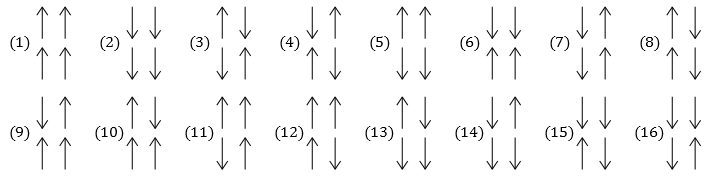
\includegraphics[width=0.75\textwidth]{Figures/Configurations.png}
	\caption{The 16 different spin configurations for the 2 dimensional case with 2 spins in each dimension. An arrow pointing upwards represents spin up with the spin value $s_{up}=+1$, whilst an arrow pointing downwards represent spin down with the spin value $s_{down}=-1$. The corresponding energies and magnetizations of each of the micro states can be found in \tabref{tab:ClosedFormSolution1}.}
	\label{fig:SpinConfigurations}
\end{figure}
The energy and magnetization for each of the $16$ microstates are given in \tabref{tab:ClosedFormSolution1} and are calculated from \matref{eq:EnergyMagnetization}. 
As an example, the energy and magnetization of the ninth microstate, given in \figref{fig:SpinConfigurations} as the state with one spin down and three spin up, is calculates here:
\begin{align*}
	E_9 &= -J \sum_{<kl>} ^{2\times 2} s_k s_l
	\\
	&= -J[((-1)\cdot 1 + (-1) \cdot 1)+(1\cdot (-1) + 1\cdot 1) + (1\cdot (-1) + 1\cdot 1 ) +(1\cdot 1 + 1\cdot 1)]
	\\
	&= 0
\end{align*}
and
\begin{align*}
	\mathcal{M} _9 = \sum _{j=1} ^{2\times 2} s_j = (-1) + 1 + 1 + 1 = 2
\end{align*}
\begin{table}[H]
\centering
\caption{Energy and magnetization of each of the spin configurations given in \figref{fig:SpinConfigurations}.}
\begin{center}
\begin{tabular}{ |l | c | c | }
  \hline			
  Configuration & Energy & Magnetization  \\
  \hline
  (1) & $-8J$ & $4$ \\
  \hline
  (2) & $-8J$ & $-4$ \\
  \hline
  (3) -- (4) & $8J$ & $0$ \\
  \hline
  (5) -- (8) & $0$ & $0$ \\
  \hline
  (9) -- (12) & $0$ & $2$ \\
  \hline
  (13) -- (16) & $0$ & $-2$ \\
  \hline
\end{tabular}
\end{center}
\label{tab:ClosedFormSolution1}
\end{table}
Hence the partition function $Z$ defined in \matref{eq:PartitionFunction} for this $2\times 2$ spin system becomes
\begin{align}
	Z = 12 + 2\left( e^{8\beta J} + e^{-8 \beta J} \right)
	= 12 + 4\cosh (8\beta J)
	\label{eq:PartitionFunction2times2}
\end{align}
In the last equation sign, Euler's identity \fxnote{ok?} and the definition of $\cosh \theta$ is used.
With this partition function and the energy and magnetization for each of the $16$ microstates given in \tabref{tab:ClosedFormSolution1}, the expectation value of the energy and the magnetization becomes
\begin{align}
	\left< E \right> = \frac{1}{Z} (-16 J e^{8\beta J} + 16 J e^{-8\beta J} )
	 = \frac{16J}{Z} (e^{-8\beta J}-e^{8\beta J})
	 \label{eq:ExpectationEnergy2times2}
\end{align} 
and
\begin{align}
	\left< \mathcal{M} \right> = \frac{1}{Z} (4e^{8\beta J} -4e^{8\beta J} +2 -2 ) = 0 
	\label{eq:ExpectationMagnetization2times2}
\end{align}
To compute the specific heat $C_v$ and the susceptibility, the quantities $\left< E^2 \right>$ and $\left< \mathcal{M}^2 \right>$ must be known.
For this $2\times 2$ spin case they become
\begin{align}
	\left< E^2 \right> = \frac{1}{Z} \sum _{i=1} ^{16} E_i ^2 e^{-\beta E_i}
	= \frac{128 J^2}{Z} (e^{8\beta J} + e^{-8\beta J} ) 
	\label{eq:ExpectationEnergySquared2times2}
\end{align}
and 
\begin{align}
	\left< \mathcal{M}^2 \right> = \frac{1}{Z} \sum _{i=1} ^{16} \mathcal{M}_i ^2 e^{-\beta E_i}
	= \frac{32}{Z} (e^{-8\beta J} + 1 ) 
	\label{eq:ExpectationMagnetizationSquared2times2}
\end{align}
The specific heat $C_v$ and the susceptibility $\chi$ can now be determined by the expressions in \matref{eq:SpecificHeatSusceptibility}, and after some joggling with the results gained by \matref{eq:ExpectationEnergy2times2}, \eqref{eq:ExpectationMagnetization2times2}, \eqref{eq:ExpectationEnergySquared2times2} and \eqref{eq:ExpectationMagnetizationSquared2times2}, it is evident that
\begin{align}
	C_v = \frac{128 J^2}{z k_B T^2} \left[ e^{8\beta J} + e^{-8\beta J} - \frac{2e^{-16\beta J}+2e^{16\beta J}+4}{Z} \right]
	\label{eq:SpecificHeat2times2}
\end{align}
\fxnote{check that this is correct}
and
\begin{align}
	\chi = \frac{16}{k_B T} (e^{-8\beta J} +1)
	\label{sec:Susceptibility2times2}
\end{align}
	\subsection{Closed Form Solutions for the $2\times 2$ case with $T=1.0$}
\label{sec:ClosedFormSolution2times2T1}
\fxnote{introduce value of partition function}
In this project, the temperature is given in the units of $[k_B T/J] = [1/\beta J]$.
To distinguish this from the temperature $T$ in the ordinary unit of Kelvin \fxnote{ok??}, the considered temperature is, in this section, written as $\tilde{T}$.
In \fxnote{ref, to section for 2x2 case}, the c++ code for computing the expectation value of the energy and the magnetization and the specific heat and susceptibility of the $2\times 2$ spin case with temperature $\tilde{T} = 1.0$ is introduced.
The section is dedicated to find the closed form solutions for these quantities for this situation with the purpose of testing the code introduced in the mentioned section. \fxnote{any ideas to improving this section??}

With $\tilde{T} = 1/\beta J = 1.0$, the partition function in \matref{eq:PartitionFunction2times2} gives the value
\begin{align}
	Z = 12+4\cosh(8) \approx 6000
\end{align}
\fxnote{write more exact result for Z}
The expectation value of the magnetization is surely still zero, whilst the expectation value of the absolute value of the magnetization becomes
\begin{align}
	\left< \mathcal{M} \right> = \frac{1}{Z} ( 8 e^8 +4) \approx 3.9926
\end{align}
With the temperature given in units of $[k_B T/J]$, the formulas for determining the expectation value of the energy and the specific heat and susceptibility, given in the previous section, must be slightly modified to give a value.
E.g. the expectation value of the energy given by \matref{eq:ExpectationEnergy2times2} will have to be divided by $J$, giving the computed expectation value in the unit of $[E/J]$. 
For a temperature of $\tilde{T} = 1.0$, the computed expectation value of the energy is then
\begin{align}
	\tilde{\left< E \right>} 
	= \frac{\left< E \right>}{J}	
	= \frac{16}{Z} (e^{-8}-e^{8}) \approx -7.9839 
\end{align} 
This is approximately the same as the lowest energy state of the system (see \tabref{tab:ClosedFormSolution1}), which is also what was to be expected for low temperatures. 
To find $C_v$ and $\chi$, \matref{eq:SpecificHeat2times2} and \eqref{sec:Susceptibility2times2} are considered, and with a temperature $\tilde{T}  = 1.0$, they give the values
\begin{align*}
	\tilde{C}_v = \frac{C_v}{J}
	\approx 0.12830
	\qquad \text{and} \qquad
	\tilde{\chi} = \chi J \approx 0.03209
\end{align*}
\fxnote{check results, especially $\chi$}
The values of the quantities gained in this section for the $2\times 2$ spin case with $\tilde{T} = 1.0$ in units of $[k_B T/J] = [1/\beta J]$ are collected in the table below.
\begin{table}[H]
\centering
\caption{Various quantity values for the $2\times 2$ spin case with temperature $\tilde{T} = 1.0$ in units of $[k_B T/J] = [1/\beta J]$.}
\begin{center}
\begin{tabular}{ | c | c | c | c | c | }
  \hline			
  $\left< \tilde{E} \right>$ & $\left< \mathcal{M} \right> $ &  $\left< |\mathcal{M} | \right> $ & $\tilde{C}_v $ & $\tilde{\chi}$  \\
  \hline
  $-7.9839$ & $0$ & $3.9926$ & $0.12830$ & $0.03209$ \\
  \hline
\end{tabular}
\end{center}
\label{tab:ClosedFormSolution2times2T1}
\end{table}
\fxnote{fix $\chi$}
	\chapter{Results and Discussion}
\label{chap:Results}
%Include your results either in figure form or in a table. Remember to label your results.
%All tables and figures should have relevant captions and labels on the axes.
write awesome introduction!

The results from running the codes bla bla bla can be found in the GitHub folder  \url{https://}.
\fxnote{fix lines!}	
	\chapter{Conclusion}
Conclude!!!!


	% ¤¤ LITTERATURLISTE: SKAL VÆRE SIDST ¤¤
		\bibliographystyle{ieeetr}
		\bibliography{Bibtex/litteratur}

% ¤¤ BILAG: SKAL VÆRE ALLERSIDST ¤¤
	\appendix

	
\end{document}
